\documentclass[11pt]{beamer}
\usetheme{Frankfurt}
\usecolortheme{rose}

\usepackage{algorithm,algorithmic}
\usepackage{hyperref}
\usepackage{url}
\usepackage{graphicx}
\usepackage{amsmath,amsthm, amssymb, latexsym}
\usepackage{bbm}
\usepackage[english]{babel}
\usepackage{epstopdf}
\usepackage{color}
\usepackage{bm}

\usefonttheme{professionalfonts}

\DeclareMathOperator*{\argmax}{arg\,max}
\DeclareMathOperator*{\argmin}{arg\,min}

\newcommand{\citecolor}[1]{({\color{blue} #1})}
\def\E{\mathbb{E}}

\newcommand\blfootnote[1]{%
  \begingroup
  \renewcommand\thefootnote{}\footnote{#1}%
  \addtocounter{footnote}{-1}%
  \endgroup
}

%Gummi|063|=)

\title[CLGP]{Deep Reinforcement Learning: Tic-Tac-Toe }
\author[Liang]{Kevin Liang}
\institute[Duke University]{Duke University}
\date{16 September 2016}
\begin{document}

\begin{frame}
\maketitle
\end{frame}



%%%%%%%%%%%%%%%%%%%%%%%%%%%%%%%%%%%%%%%%%%%%%%%%%%%%%%%
\section{Introduction}

\subsection{Introduction}
\begin{frame}{Introduction}
	\begin{itemize}
	
		\item Goal: Have an agent learn how to play Tic-tac-Toe using deep reinforcement learning 
		\item Tic-Tac-Toe game
		\begin{itemize}
			\item Players X and O take turns placing marks on a 3x3 grid
			\item Player that achieves a 3-in-a-row wins
			\item If the board fills up without a winner: draw
		\end{itemize}
		\item Toy example to get started before tackling more complicated settings (eg. Atari games of OpenAI Gym)
		
	\end{itemize}
\end{frame}

\section{Agents}

\subsection{Agent 1}
\begin{frame}{Agent 1: Deep Reinforcement Learner}
	\begin{minipage}[t]{0.55\linewidth}
		\begin{itemize}
			\item Agent is given a 64x64 image of the state of the board, not the 3x3 state space directly.
			\item Agent not informed of rules. Does not know:
				\begin{itemize}
					\item what leads to a win/loss
					\item own identity
					\item marking an already occupied spot is an illegal move
				\end{itemize}
			\item Use direct policy search (policy gradients) to update weights
			\item Action stochasticity: multinomial distribution
		\end{itemize}
	\end{minipage}
	\hfill
	\begin{minipage}[t]{0.4\linewidth}
		\centering
		\begin{figure}[tttDL]
			\centering
			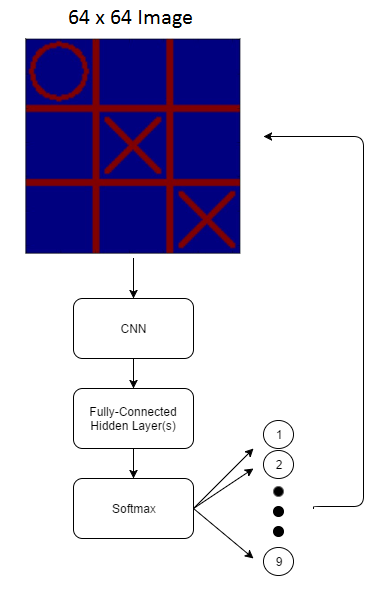
\includegraphics[width=.95\textwidth]{Figures/deeptictactoe.png}
		\end{figure}
	\end{minipage}
\end{frame}

\begin{frame}{Agent 1: Architecture}
	\begin{minipage}[t]{0.68\linewidth}
		\begin{itemize}
			\item Input: 64x64 image
			\item CNN: 8  x (3,3), ReLU
			\item[] CNN: 16 x (3,3), ReLU
			\item[] MaxPool: (2,2)
			\item CNN: 16 x (3,3), ReLU
			\item[] CNN: 16 x (3,3), ReLU
			\item[] MaxPool: (2,2)
			\item CNN: 16 x (3,3), ReLU
			\item[] CNN: 16 x (3,3), ReLU
			\item[] MaxPool: (2,2)
			\item Fully Connected: 16 x 8x8 $\rightarrow$ 30, ReLU
			\item Fully Connected: 30 $\rightarrow$ 9
			\item Softmax
		\end{itemize}
	\end{minipage}
	\hfill
	\begin{minipage}[t]{0.3\linewidth}
		\centering
		\begin{figure}[tttDL]
			\centering
			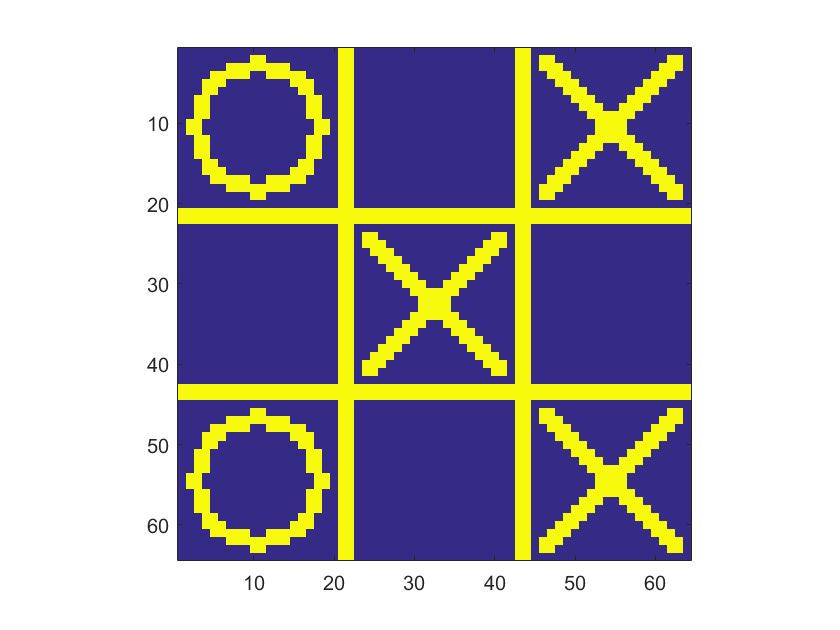
\includegraphics[width=1.5\textwidth]{Figures/boardExample.png}
		\end{figure}
	\end{minipage}
\end{frame}

\subsection{Agent 2}
\begin{frame}{Agent 2: "Optimal" opponent}	
	\begin{minipage}[t]{0.55\linewidth}
		\begin{itemize}
			\item Agent is given the 3x3 state space directly.
			\item Agent knows rules. Knows:
			\begin{itemize}
				\item what leads to a win/loss
				\item own identity
				\item marking an already occupied spot is an illegal move
			\end{itemize}
			\item Add a "difficulty" parameter that controls how often the "optimal" agent makes a random (legal) move, instead of always following rules
			\begin{itemize}
				\item Allows for the deep RL agent to occasionally win
			\end{itemize}	
		\end{itemize}
	\end{minipage}
	\hfill
	\begin{minipage}[t]{0.4\linewidth}
		\centering
		\begin{figure}[tttAI]
			\centering
			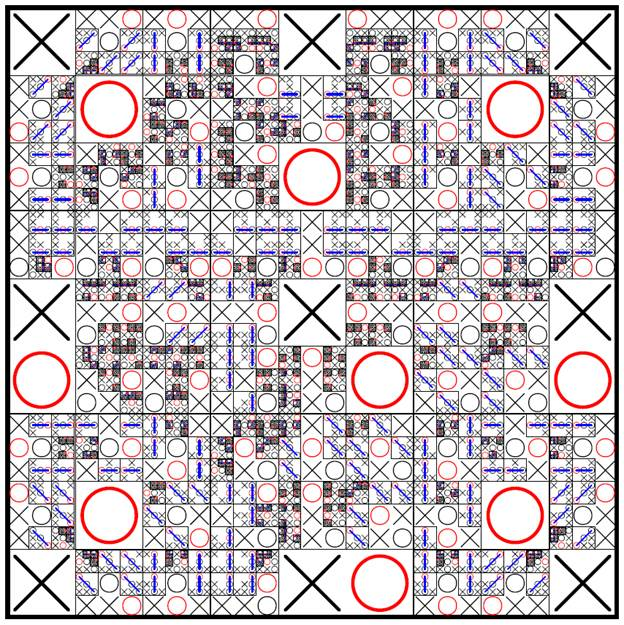
\includegraphics[width=.95\textwidth]{Figures/tttAI.jpg}
		\end{figure}
	\end{minipage}
\end{frame}

\begin{frame}{Agent 2: "Architecture"}
	Newell and Simon Tic-Tac-Toe Rules:
	\begin{itemize}
		\item Rule 1: If agent can win, then make a 3-in-a-row
		\item Rule 2: If opponent can win, block the winning move
		\item Rule 3: Make a fork (two 2-in-a-rows)
		\item Rule 4: Block an opponent's fork, while simultaneously making a 2-in-a-row if possible
		\item Rule 5: Take the center
		\item Rule 6: If opponent has a corner, take the opposite corner
		\item Rule 7: Take an empty corner
		\item Rule 8: Take an empty side
	\end{itemize}		
\end{frame}



\section{Reinforcement Learning}

\subsection{Set-up}
\begin{frame}{Reinforcement Learning Set-up - Agent 1's perspective}
	\begin{itemize}
		% Add an image of the board here
		\item {\it State}: 64x64 image of the board
		\item {\it Action}: 1 of 9 moves corresponding to the 9 spaces on the board
		\item {\it Reward}: Given at the end of a game. One of four outcomes:
		\begin{itemize}
			\item Win: {\it +1} - The agent successfully made 3-in-a-row 
			\item Draw: {\it 0} - The board filled up without either player winning
			\item Loss: {\it -1} - The opponent made 3-in-a-row
			\item Broken: {\it -10} - The agent broke a rule by trying to play a symbol where one already had been placed
		\end{itemize}
	\end{itemize}
\end{frame}

\begin{frame}{Training Regimen}
%	\begin{algorithm}
%		\caption{Training Deep Agent}
%		\begin{algorithmic}[1]
%			\STATE Initialize net params $\bm \theta$ randomly
%			\WHILE{not converged}
%				\STATE Initialize images $\bm x$, actions $\bm a$, labels $\bm l$, durations $\bm t$, player identities $\bm z$ to empty
%				\FOR{$k = 1$ \TO M }
%					\STATE Play game with $\bm \theta$ held constant
%					\IF Broken Rule
%						\STATE Discard all but last frame
%					\ENDIF
%					\STATE Append frames of game k to $\bm x$, $\bm a$, $\bm l$, $\bm t$, $\bm z$
%				\ENDFOR
%				\STATE {\it loss} $= f(\bm x, \bm a, \bm l, \bm t, \bm z)$
%				\STATE $\bm \theta = $ ADAM({\it loss},$\bm \theta$)
%			\ENDWHILE
%		\end{algorithmic}
%	\end{algorithm}
\end{frame}

\begin{frame}[shrink=15]{Loss Expression}
	Player 1: Deep Reinforcement Learner \qquad \qquad Player 2: Optimal Player \\
	\vspace{5 mm}
	\begin{itemize}
		\item Loss for Player $j$, $j \in \{1,2\}$:
		\begin{equation}
		loss_j = -\frac{1}{N} \sum_{i \in z_i=j} \gamma^{t_i} p(y_i=a_i|x_i) r_{l_i} 
		\end{equation}
		\item Total loss (zero-sum game):
		\begin{equation}
		loss = loss_1 - loss_2
		\end{equation}
	\end{itemize}
	
	\begin{align*}
		x_i &= \text{image of board in frame } i & y_i &= \text{output of network softmax after frame } i \\
		a_i &= \text{action taken after frame } i  & l_i &= \text{eventual game result $(W,D,L,B)$ of frame } i \\
		r_l &= \text{reward of game result } l & t_i &= \text{duration of game that frame } i \text{ is part of} \\
		z_i &= \text{player presented with frame } i & \gamma &= \text{discount factor} \\
		N &= \#\text{ of frames in training set}
	\end{align*}	
\end{frame}

\subsection{Results}
\begin{frame}{Results - AI.X = 0.5; AI.O = 0.6}
	\begin{figure}[Results]
		\centering
		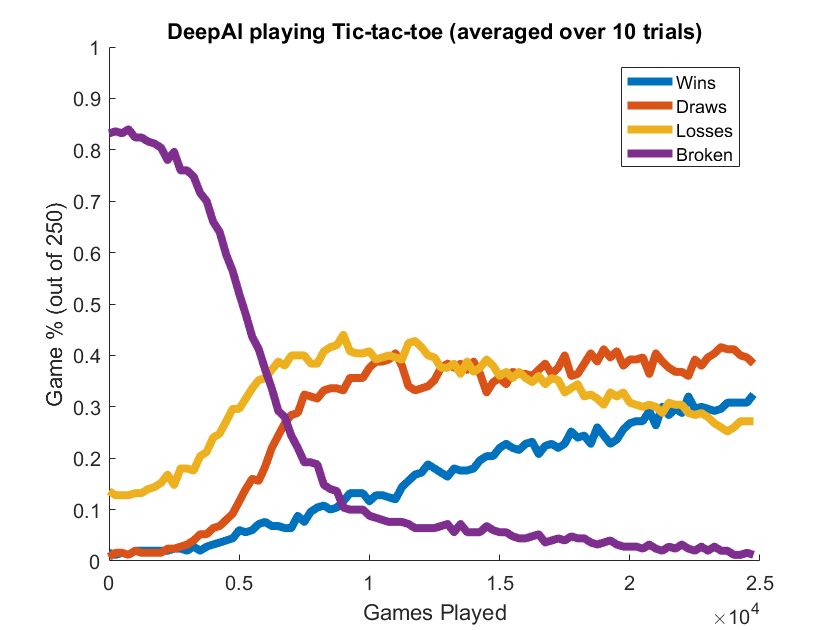
\includegraphics[width=0.95\textwidth]{Figures/results05X06O.png}
	\end{figure}
\end{frame}

\subsection{Next Steps}
\begin{frame}{Next Steps}
	\begin{itemize}
		\item DGDN Decoder to utilize discarded broken frames
		\item Knowledge transfer to other tasks: 
		\begin{itemize}
			\item Digital Mammography DREAM Challenge
			\item TSA Airport Scanners
		\end{itemize}
		\item Future RL explorations (and exploitations)
	\end{itemize}
\end{frame}

\end{document}
